\chapter{Circuits}
\label{chap:circuits}
For measuring the response of a pressure-sensitive film, a circuit should be formed to obtain stable and accurate measurements. A sensor is commonly drawing power from the circuits power source. This can lead to current drops under initial loading of the sensor. This is a common observed phenomena which can introduce inaccuracies in the voltage output. An operational amplifier circuit will come to great benefit when sensors are introduced. The operational amplifier is equipped with an external power source for the sensor to draw power from. More details on the alternative circuits are investigated in the following sections.

\section{Voltage divider}
\label{sec:vd}
A voltage divider is one of the simplest forms of circuits (Figure \ref{fig:voltagedivider}) considered for a pressure-sensitive film. The quality of the measurement result is based on the voltage read from the circuit. The voltage varies when the resistance of the sensor changes due to applied force. This voltage is based on the analytic formula: 
\begin{equation}
\label{eq:voltagedivider}
    V_{out} = V_{supply} \cdot \frac{R_1}{R_{flexiforce} + R_1}
\end{equation}
\begin{figure*}[!b]
    \centering
    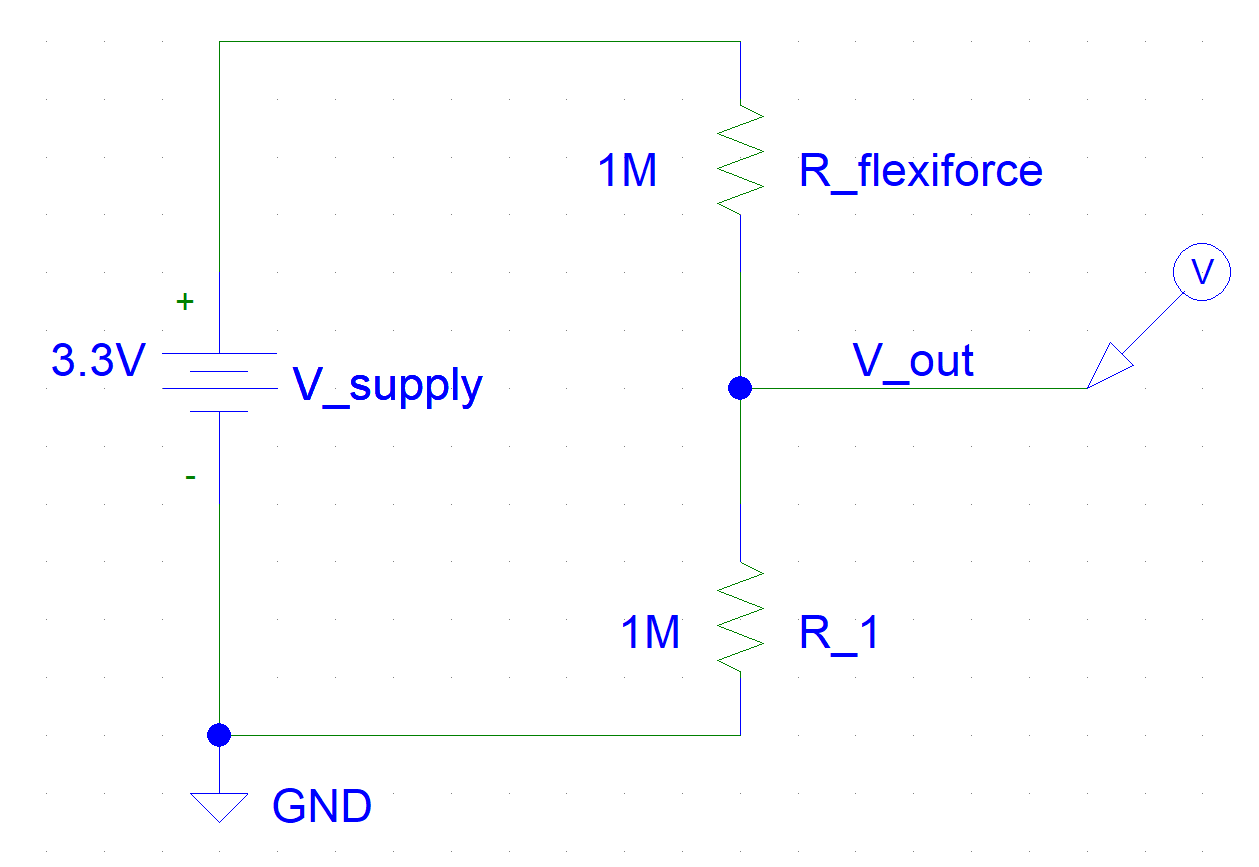
\includegraphics[width=.985\linewidth]{figures/voltage_divider.png}
    \caption{Voltage divider circuit for sensing changes in pressure sensitive films (created in PSpice)}
    \label{fig:voltagedivider}
\end{figure*}
When applying pressure on the sensor, the resistance decreases, resulting in an increase in voltage in $V_{out}$.  One of the benefits of using a voltage divider, is the easy implementation. On the contrary, we can experience more interference in the measured voltage and measurement spike due to the sensor drawing power straight from the power source. !Kg formula

\section{Operational amplifier circuits}
\label{sec:opamps}
Operational amplifiers are 3 terminal devices used to amplify voltages, two inputs and one output, with an addition of two power connections ($V_{supply}$). These so called OP-amps are described to have infinite input impedance, meaning it has infinite resistance on the two inputs, hindering current flow between the inputs and a zero output impedance. This is the case for ideal Op-amps, where in the real world applications, no Op-amp is perfect and some variations in current and voltage may occur. Operational amplifiers can be connected in two main forms of circuits, the \textit{Inverting operational amplifier circuit} and \textit{Non-inverting operational amplifier circuit}. By leaving the two inputs open, the ideal operational amplifier is defined to be in a "Open-loop"-state, resulting in infinite gain (A) and bandwidth. In real world applications, the gain can be adjusted by increasing or decreasing the feedback- or input-resistance and is a measure of how good a operational amplifier is. The power connectors on the operational amplifier is defined as $V_{supply}$, which decides the operational voltage range of the amplifier. This operational voltage range usually caps at $\pm 15V$, which gives us a upper limit of how much the circuit is able to amplify a current to.

\subsection{Inverting Operational amplifier circuit}
\label{subsec:invopamp}
The inverting operational amplifier (Figure \ref{fig:invertingopamp}) is based on the characteristics described in Section \ref{sec:opamps}. This circuit is based on a negative feedback connection of the two inputs available. This results in an amplified signal with a negative sign, giving an overall reduced amplification. In this case, the pressure sensitive film, is connected as the $R_{in}$ resistor, which allows the output voltage $V_{out}$ to vary from $0V$ to $-V_{supply}$, and for a biased input, it can vary from $V_{bias}$ down to $0V$. When applying force to the sensor, resistance decreases and voltage on the output increases (Equation \ref{eq:invopamp_amplifier_vout}).

\begin{equation}
\label{eq:invopamp_amplifier}
    A = \frac{V_{out}}{V_{in}} = - \frac{R_{feedback}}{R_{flexiforce}}
\end{equation}

\begin{equation}
\label{eq:invopamp_amplifier_vout}
    V_{out}= -V_{in} \cdot \frac{R_{feedback}}{R_{flexiforce}}
\end{equation}

\begin{figure*}
    \centering
    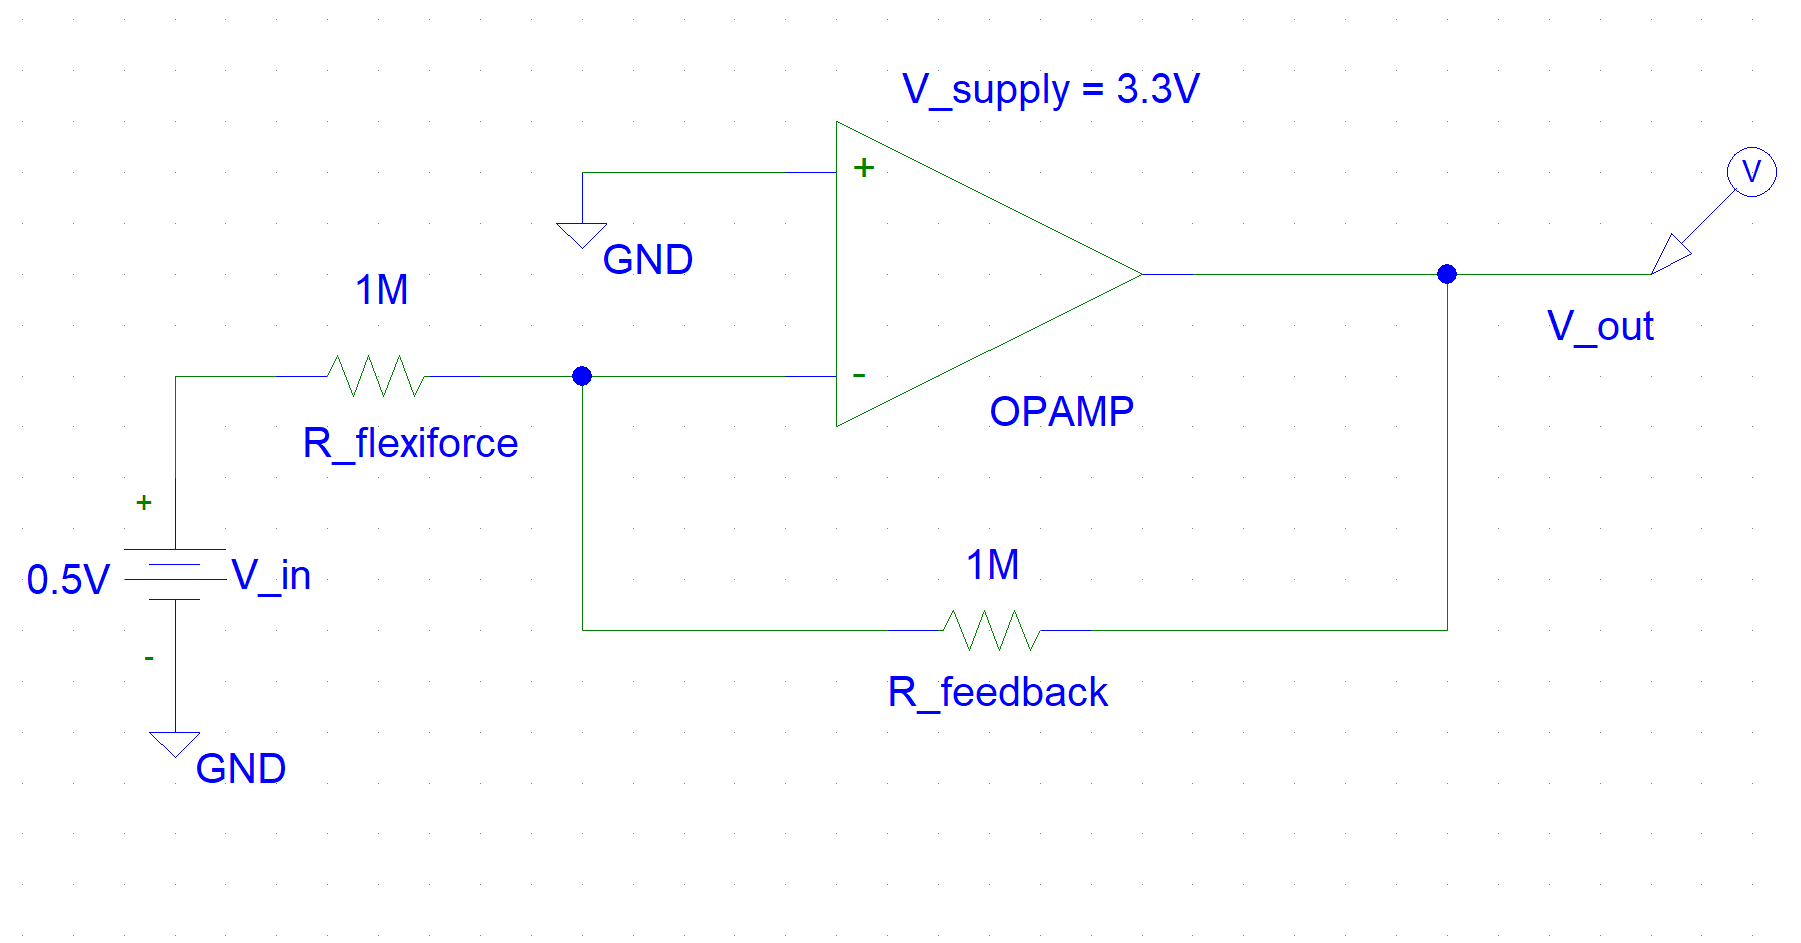
\includegraphics[width=.985\linewidth]{figures/inverting_opamp.png}
    \caption{Inverting operational amplifier circuit for sensing changes in pressure sensitive films, in unity state A=1. (created in PSpice)}
    \label{fig:invertingopamp}
\end{figure*}


\subsection{Non-inverting operational amplifier circuit}
\label{subsec:noninvopamp}
Much like the Inverting operational amplifier, the non-inverting version (positive feedback) connects its feedback to the negative input on the op-amp, but is running voltage input on the positive side. With the addition of feedback running to ground (Figure \ref{fig:noninvertingopamp}). The effect of using a non-inverting operational amplifier circuit is an overall increase in gain compared to the inverting op-amp circuit. Due to the overall increase in amplification, seen from Equation \ref{eq:noninvopamp_amplifier_vout}, one can experience instabilities in the output for lower values of voltage (micro volts).
\begin{equation}
\label{eq:noninvopamp_amplifier}
    A = \frac{V_{out}}{V_{in}} = 1 + \frac{R_{feedback}}{R_{flexiforce}}
\end{equation}

\begin{equation}
\label{eq:noninvopamp_amplifier_vout}
    V_{out} = V_{in}(1 + \frac{R_{feedback}}{R_{flexiforce}})
\end{equation}

\begin{figure*}
    \centering
    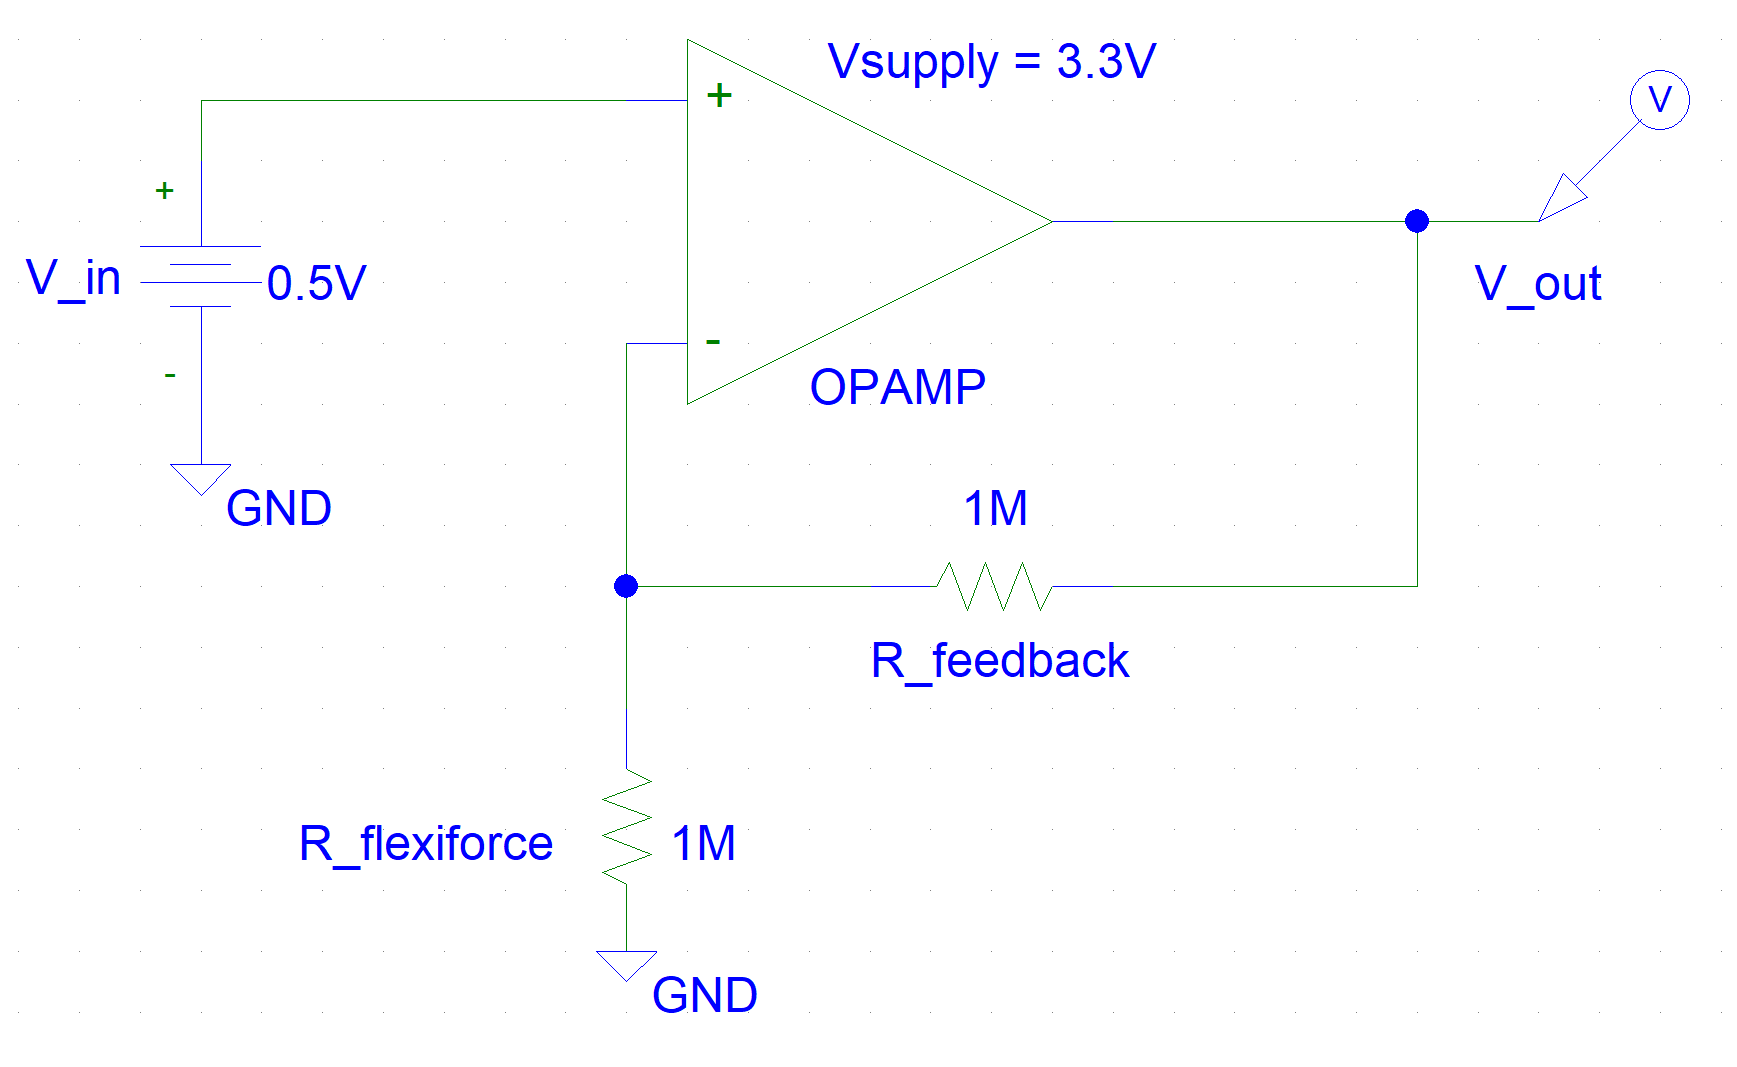
\includegraphics[width=.985\linewidth]{figures/noninverting_opamp.png}
    \caption{Non-inverting operational amplifier circuit for sensing changes in pressure sensitive films (created in PSpice)}
    \label{fig:noninvertingopamp}
\end{figure*}

\section{Implementation of a capacitors}
\label{sec:capacitor}
When it comes to implementing a analog low-pass filter, a capacitor in parallel with the feedback resistance is implemented in the operational amplifier circuits (Figure \ref{fig:capacitor}) as a first order low-pass filter. One would see this as an option to deal with high frequency spikes in the measurements. The capacitors function in parallel with a resistor, is to filter out higher frequencies, dependent on the size of the capacitor. When the capacitor reaches its cutoff frequency $\omega$, it causes a short in the circuit, leading all frequencies higher than the cutoff frequency to ground or a specified point in the circuit. A larger capacitor will have lower higher cutoff frequency as defined in Equation \ref{eq:cutoff}. By introducing the capacitor, it causes an extra pole in the frequency response of the amplifier circuit, making it more stable. Additionally, introducing capacitors by the power supply and the output of the circuit, additional means of fighting noise in the circuit is introduced.

\begin{equation}
\label{eq:cutoff}
    \omega = \frac{1}{R_{feedback}C_1}
\end{equation}

\begin{figure*}
    \centering
    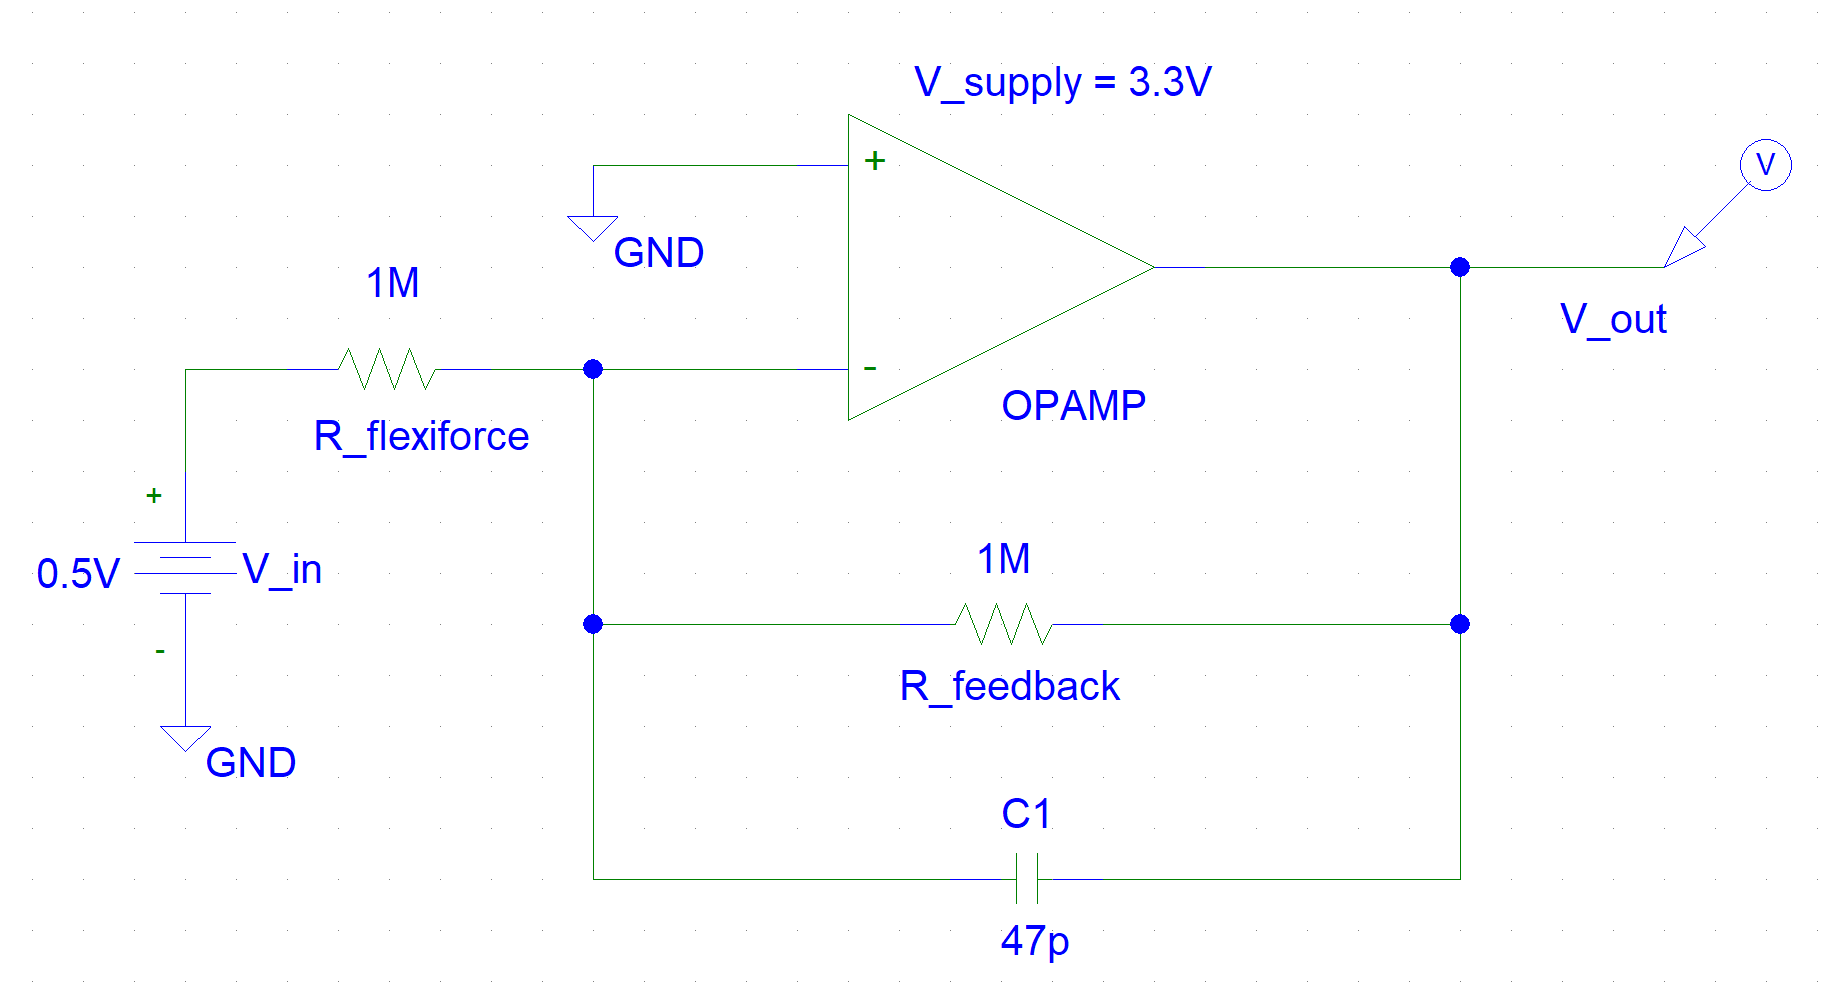
\includegraphics[width=.985\linewidth]{figures/capacitor.png}
    \caption{Inverting operational amplifier circuit with capacitor (created in PSpice)}
    \label{fig:capacitor}
\end{figure*}

\section{Simulating the circuits}
\label{sec:simulation}
The simulation of the alternative circuits was an important mean in designing and tuning the circuits. It was first and foremost important to look at the circuits behavior under ideal condition to understand how they would perform, in terms of output voltage. By simulation, the appropriate resistance values for resistors could be found. PSpice was the first simulation program for initial tests of functionality, were LTSpice was later used for 
\subsection{LTSpice}
\label{subsec:ltspice}

\subsection{PSpice}
\label{subsec:pspice}


\section{Chapter results}
\label{sec:circuitresults}

Several tests on the two circuits were conducted using an Arduino UNO microcontroller \ref{sec:arduinouno}. Each test consisted of 1000 samples for each circuit. To investigate the differences in measurement quality and noise handling, the Flexiforce A201 sensor was loaded with $200g$ and $500g$ calibration weights (Figure \ref{fig:opamp_test200} \& \ref{fig:opamp_test500}).

\begin{figure}[!htb]
   \begin{minipage}{0.470\textwidth}
     \centering
     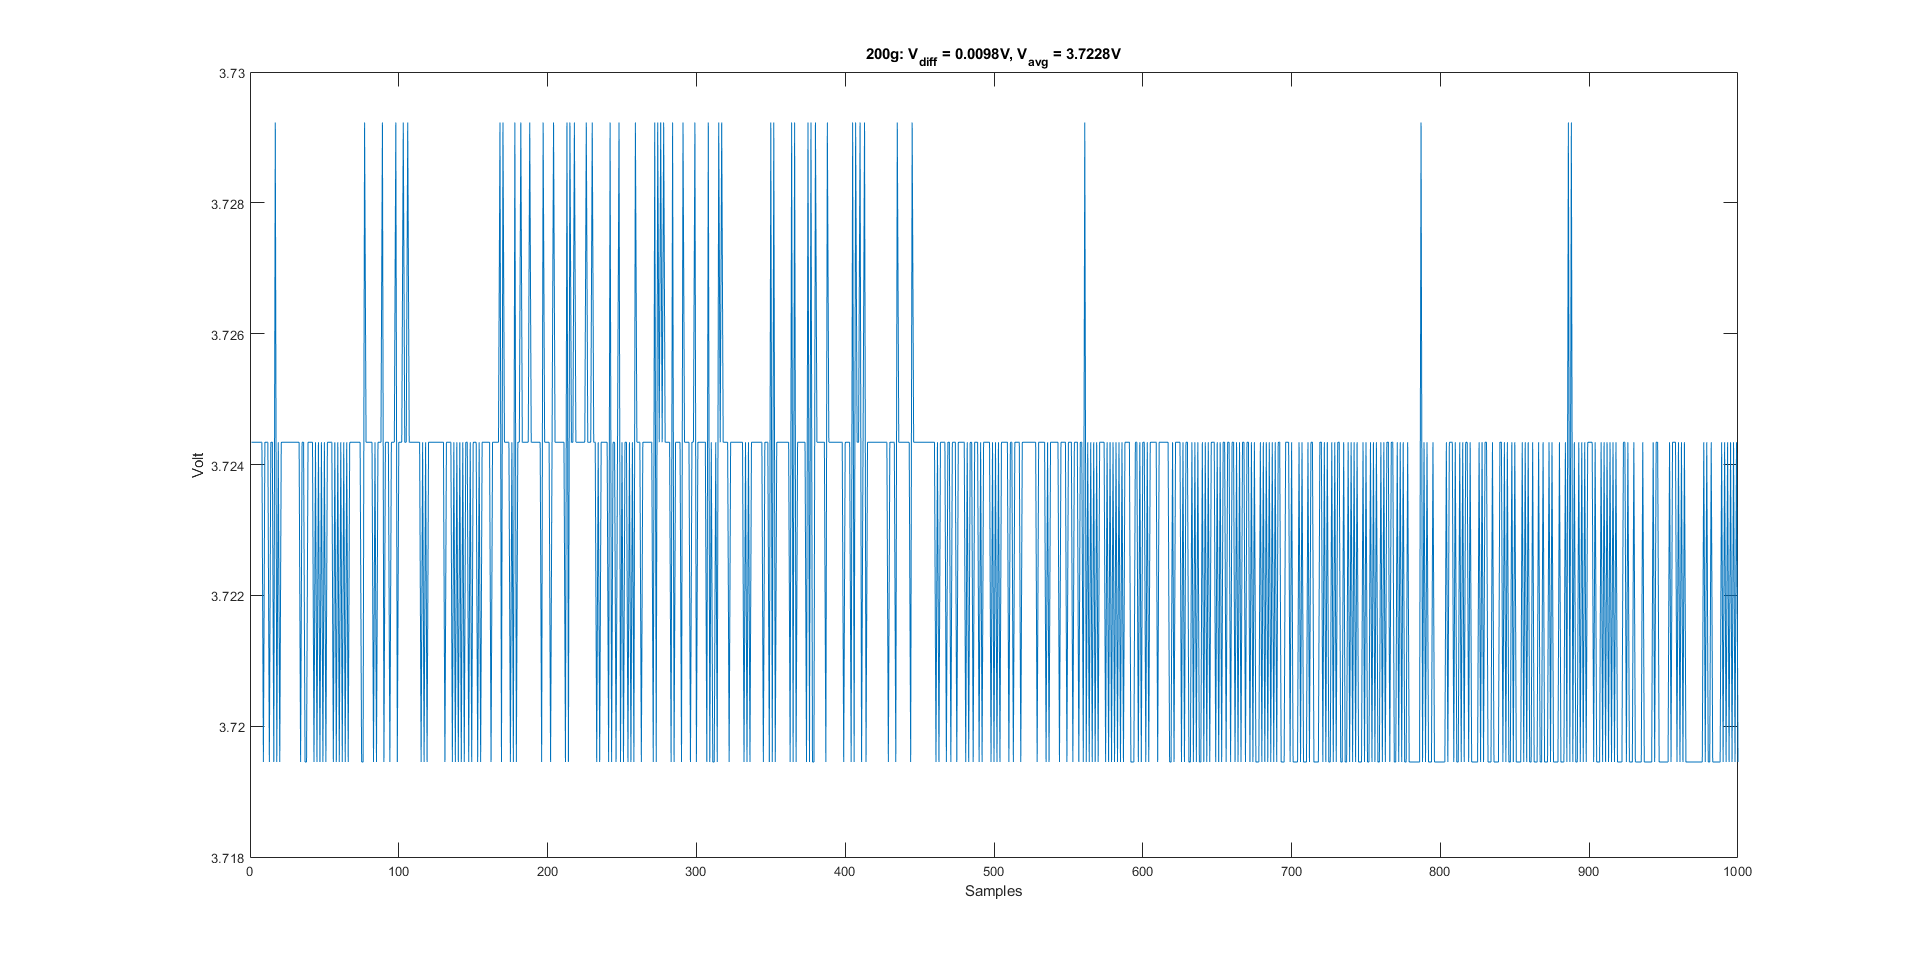
\includegraphics[width=0.7\textwidth]{figures/opamp_Vdiff_200g.png}
     \caption{1000 samples of 200g test for operational amplifier}
     \label{fig:opamp_test200}
   \end{minipage}\hfill
   \begin{minipage}{0.470\textwidth}
     \centering
     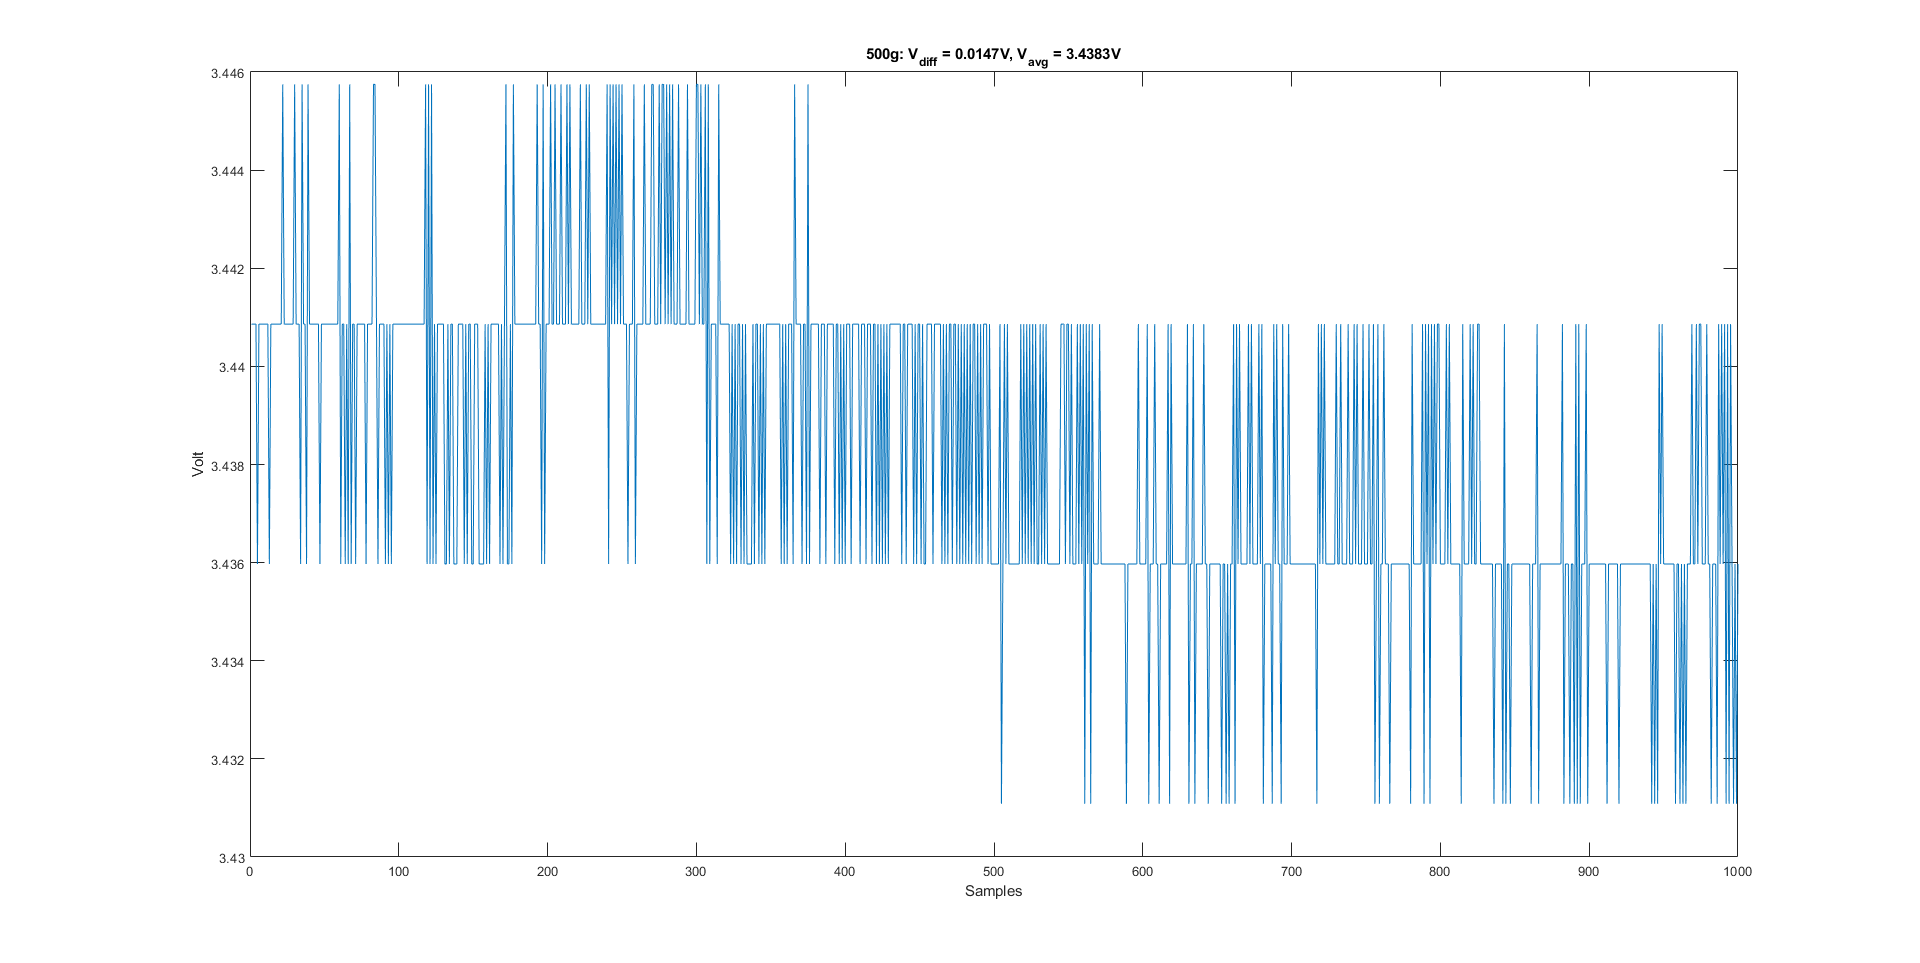
\includegraphics[width=0.7\textwidth]{figures/opamp_Vdiff_500g.png}
     \caption{500 sampling test for operational amplifier circuit with 500g weight, analysing voltage variation}
     \label{fig:opamp_test500}
   \end{minipage}
\end{figure}




\section{Chapter discussion}
\label{sec:circuitdisc}
In the process of selecting a force sensing sensor, it is required to chose the most suited sensor for the application area. In the research done by Fabrizio Vecchi and his colleagues \citep{vecchi_experimental_2000} on commercial sensors in biomechanics and motorcontrol, sensors like the \textit{Flexiforce A201 \ref{sec:flexiforce}} and \textit{Force Sensing Resistor \ref{sec:interlink}} were evaluated. In terms of linearity, time-drift tests and robustness, the Flexiforce sensor presented better results. As mentioned, the application area is what determines the choice of sensor, and for this thesis a sensor is required for handling forces significantly higher than the research conducted by Vecchi et. al (2000). The Flexiforce sensor in combination with the operational amplifier circuits prove to show similar results in terms of linearity, which is a key factor to obtain consistent and accurate results in measurements. After analysing the voltage divider and operational amplifier circuits, a clear difference in terms of noise and measurement spikes were observed. The operational amplifier circuit \ref{sec:opamps} proved to reduce the variation of voltage over time (Figur \ref{fig:opamp_test200} \& \ref{fig:opamp_test500}).


Needed weight to measure (45/4) osv.

\section{Summary}
\label{sec:circuitsummary}
Sensors and circuits presented in Section \ref{chap:sensors} and \ref{chap:circuits}, the linearity and consistency of measurements were tested and evaluated. Differences were found in terms of noise (measurement spikes and variance), linearity and precision. An operational amplifier circuit was selected reasoned by the requirement of precise measurements and linearity with low-noise outputs and low-power consumption. In combination with the Flexiforce A201 sensor, the system was able to handle the required forces up to 450\si{\newton} (or 45-46\si{\kilogram}). As suggested by Tekscan, Inc., a inverting operational amplifier circuit was chosen.
External and internal noise were handled by implementing a capacitor as a analog low pass filter, which proved to have a positive effect on the quality of the sampled data.
\begin{itemize}
    \item \textbf{!! How I calibrated and why}
\end{itemize}

